% -*- Mode:TeX -*-

%% IMPORTANT: The official thesis specifications are available at:
%%            http://libraries.mit.edu/archives/thesis-specs/
%%
%%            Please verify your thesis' formatting and copyright
%%            assignment before submission.  If you notice any
%%            discrepancies between these templates and the 
%%            MIT Libraries' specs, please let us know
%%            by e-mailing thesis@mit.edu

%% The documentclass options along with the pagestyle can be used to generate
%% a technical report, a draft copy, or a regular thesis.  You may need to
%% re-specify the pagestyle after you \include  cover.tex.  For more
%% information, see the first few lines of mitthesis.cls. 

%\documentclass[12pt,vi,twoside]{mitthesis}
%%
%%  If you want your thesis copyright to you instead of MIT, use the
%%  ``vi'' option, as above.
%%
%\documentclass[12pt,twoside,leftblank]{mitthesis}
%%
%% If you want blank pages before new chapters to be labelled ``This
%% Page Intentionally Left Blank'', use the ``leftblank'' option, as
%% above. 

\documentclass[12pt,twoside]{mitthesis}
\usepackage{lgrind}
\usepackage{amssymb}
\usepackage{amsmath}
\usepackage{amsthm}
\usepackage{graphicx}
\usepackage{xcolor}
%% These have been added at the request of the MIT Libraries, because
%% some PDF conversions mess up the ligatures.  -LB, 1/22/2014
\usepackage{cmap}
\usepackage[T1]{fontenc}

\allowdisplaybreaks

\newtheorem{theorem}{THEOREM}[chapter]
\newtheorem{corollary}{COROLLARY}[theorem]
\newtheorem{lemma}[theorem]{LEMMA}

\theoremstyle{proposition}
\newtheorem{proposition}{PROPOSITION}[chapter]

\theoremstyle{remark}
\newtheorem{remark}{REMAEK}[chapter]

\theoremstyle{definition}
\newtheorem{definition}{DEFINITION}[chapter]

\newcommand\tobeclarified[1]{\textcolor{red}{#1}}

\pagestyle{plain}

%% This bit allows you to either specify only the files which you wish to
%% process, or `all' to process all files which you \include.
%% Krishna Sethuraman (1990).

\typein [\files]{Enter file names to process, (chap1,chap2 ...), or `all' to
process all files:}
\def\all{all}
\ifx\files\all \typeout{Including all files.} \else \typeout{Including only \files.} \includeonly{\files} \fi

\begin{document}

% -*-latex-*-
% 
% For questions, comments, concerns or complaints:
% thesis@mit.edu
% 
%
% $Log: cover.tex,v $
% Revision 1.8  2008/05/13 15:02:15  jdreed
% Degree month is June, not May.  Added note about prevdegrees.
% Arthur Smith's title updated
%
% Revision 1.7  2001/02/08 18:53:16  boojum
% changed some \newpages to \cleardoublepages
%
% Revision 1.6  1999/10/21 14:49:31  boojum
% changed comment referring to documentstyle
%
% Revision 1.5  1999/10/21 14:39:04  boojum
% *** empty log message ***
%
% Revision 1.4  1997/04/18  17:54:10  othomas
% added page numbers on abstract and cover, and made 1 abstract
% page the default rather than 2.  (anne hunter tells me this
% is the new institute standard.)
%
% Revision 1.4  1997/04/18  17:54:10  othomas
% added page numbers on abstract and cover, and made 1 abstract
% page the default rather than 2.  (anne hunter tells me this
% is the new institute standard.)
%
% Revision 1.3  93/05/17  17:06:29  starflt
% Added acknowledgements section (suggested by tompalka)
% 
% Revision 1.2  92/04/22  13:13:13  epeisach
% Fixes for 1991 course 6 requirements
% Phrase "and to grant others the right to do so" has been added to 
% permission clause
% Second copy of abstract is not counted as separate pages so numbering works
% out
% 
% Revision 1.1  92/04/22  13:08:20  epeisach

% NOTE:
% These templates make an effort to conform to the MIT Thesis specifications,
% however the specifications can change.  We recommend that you verify the
% layout of your title page with your thesis advisor and/or the MIT 
% Libraries before printing your final copy.
\title{q-TASEP From the Duality Approach}

\author{Wang Kunzhen}
% If you wish to list your previous degrees on the cover page, use the 
% previous degrees command:
%       \prevdegrees{A.A., Harvard University (1985)}
% You can use the \\ command to list multiple previous degrees
%       \prevdegrees{B.S., University of California (1978) \\
%                    S.M., Massachusetts Institute of Technology (1981)}
\department{Department of Mathematics, Faculty of Science}


\homefaculty{Department of Computer Science, School of Computing}

% If the thesis is for two degrees simultaneously, list them both
% separated by \and like this:
% \degree{Doctor of Philosophy \and Master of Science}
\degree{Bachelor of Science (Hons) in Applied Mathematics}

% As of the 2007-08 academic year, valid degree months are September, 
% February, or June.  The default is June.
\degreemonth{March}
\degreeyear{2016}
\thesisdate{March, 2016}

%% By default, the thesis will be copyrighted to MIT.  If you need to copyright
%% the thesis to yourself, just specify the `vi' documentclass option.  If for
%% some reason you want to exactly specify the copyright notice text, you can
%% use the \copyrightnoticetext command.  
%\copyrightnoticetext{\copyright IBM, 1990.  Do not open till Xmas.}

% If there is more than one supervisor, use the \supervisor command
% once for each.
\supervisor{Wang Dong}{Assistant Professor}

% This is the department committee chairman, not the thesis committee
% chairman.  You should replace this with your Department's Committee
% Chairman.
%\chairman{Arthur C. Smith}{Chairman, Department Committee on Graduate Theses}

% Make the titlepage based on the above information.  If you need
% something special and can't use the standard form, you can specify
% the exact text of the titlepage yourself.  Put it in a titlepage
% environment and leave blank lines where you want vertical space.
% The spaces will be adjusted to fill the entire page.  The dotted
% lines for the signatures are made with the \signature command.
\maketitle

% The abstractpage environment sets up everything on the page except
% the text itself.  The title and other header material are put at the
% top of the page, and the supervisors are listed at the bottom.  A
% new page is begun both before and after.  Of course, an abstract may
% be more than one page itself.  If you need more control over the
% format of the page, you can use the abstract environment, which puts
% the word "Abstract" at the beginning and single spaces its text.

%% You can either \input (*not* \include) your abstract file, or you can put
%% the text of the abstract directly between the \begin{abstractpage} and
%% \end{abstractpage} commands.

% First copy: start a new page, and save the page number.
\cleardoublepage
% Uncomment the next line if you do NOT want a page number on your
% abstract and acknowledgments pages.
% \pagestyle{empty}
\setcounter{savepage}{\thepage}
\begin{abstractpage}
% $Log: abstract.tex,v $
% Revision 1.1  93/05/14  14:56:25  starflt
% Initial revision
% 
% Revision 1.1  90/05/04  10:41:01  lwvanels
% Initial revision
% 
%
%% The text of your abstract and nothing else (other than comments) goes here.
%% It will be single-spaced and the rest of the text that is supposed to go on
%% the abstract page will be generated by the abstractpage environment.  This
%% file should be \input (not \include 'd) from cover.tex.
In this thesis, I studied the model q-TASEP from the duality approach with main reference to the two papers \cite{duality2014} and \cite{asymptotics2013}. An ansatz explicit formula for the expectation of q-Laplace transform of the probability function describing the position of a particular particle at any time in the future in form of the nested contour integral will be provided. After this, I worked to transform a generating function of the nested contour integrals to the form of a Fredholm determinant using both the Mellin-Barnes type approach and the Cauchy-type approach. The thesis is then concluded with an asymptotic analysis on the behaviour of the rescaled fluctuation of a particular particle around its macroscopic position.
\end{abstractpage}

% Additional copy: start a new page, and reset the page number.  This way,
% the second copy of the abstract is not counted as separate pages.
% Uncomment the next 6 lines if you need two copies of the abstract
% page.
% \setcounter{page}{\thesavepage}
% \begin{abstractpage}
% % $Log: abstract.tex,v $
% Revision 1.1  93/05/14  14:56:25  starflt
% Initial revision
% 
% Revision 1.1  90/05/04  10:41:01  lwvanels
% Initial revision
% 
%
%% The text of your abstract and nothing else (other than comments) goes here.
%% It will be single-spaced and the rest of the text that is supposed to go on
%% the abstract page will be generated by the abstractpage environment.  This
%% file should be \input (not \include 'd) from cover.tex.
In this thesis, I studied the model q-TASEP from the duality approach with main reference to the two papers \cite{duality2014} and \cite{asymptotics2013}. An ansatz explicit formula for the expectation of q-Laplace transform of the probability function describing the position of a particular particle at any time in the future in form of the nested contour integral will be provided. After this, I worked to transform a generating function of the nested contour integrals to the form of a Fredholm determinant using both the Mellin-Barnes type approach and the Cauchy-type approach. The thesis is then concluded with an asymptotic analysis on the behaviour of the rescaled fluctuation of a particular particle around its macroscopic position.
% \end{abstractpage}

\cleardoublepage

\section*{Acknowledgments}

I would like to take the opportunity to express my special thanks to my supervisor, Professor Wang Dong, for his extraordinary support and assisstance extended to me for whole the year.

%%%%%%%%%%%%%%%%%%%%%%%%%%%%%%%%%%%%%%%%%%%%%%%%%%%%%%%%%%%%%%%%%%%%%%
% -*-latex-*-

% Some departments (e.g. 5) require an additional signature page.  See
% signature.tex for more information and uncomment the following line if
% applicable.
% % -*- Mode:TeX -*-
%
% Some departments (e.g. Chemistry) require an additional cover page
% with signatures of the thesis committee.  Please check with your
% thesis advisor or other appropriate person to determine if such a 
% page is required for your thesis.  
%
% If you choose not to use the "titlepage" environment, a \newpage
% commands, and several \vspace{\fill} commands may be necessary to
% achieve the required spacing.  The \signature command is defined in
% the "mitthesis" class
%
% The following sample appears courtesy of Ben Kaduk <kaduk@mit.edu> and
% was used in his June 2012 doctoral thesis in Chemistry. 

\begin{titlepage}
\begin{large}
This doctoral thesis has been examined by a Committee of the Department
of Chemistry as follows:

\signature{Professor Jianshu Cao}{Chairman, Thesis Committee \\
   Professor of Chemistry}

\signature{Professor Troy Van Voorhis}{Thesis Supervisor \\
   Associate Professor of Chemistry}

\signature{Professor Robert W. Field}{Member, Thesis Committee \\
   Haslam and Dewey Professor of Chemistry}
\end{large}
\end{titlepage}


\pagestyle{plain}
  % -*- Mode:TeX -*-
%% This file simply contains the commands that actually generate the table of
%% contents and lists of figures and tables.  You can omit any or all of
%% these files by simply taking out the appropriate command.  For more
%% information on these files, see appendix C.3.3 of the LaTeX manual. 
\tableofcontents
\newpage
\listoffigures
\newpage
\listoftables


%% This is an example first chapter.  You should put chapter/appendix that you
%% write into a separate file, and add a line \include{yourfilename} to
%% main.tex, where `yourfilename.tex' is the name of the chapter/appendix file.
%% You can process specific files by typing their names in at the 
%% \files=
%% prompt when you run the file main.tex through LaTeX.
\chapter{Introduction}
In this thesis I studied a 1-dimensional interacting particle system model called q-TASEP. It's one of the most recently yet classical particle model in this field that has important application in the physical world. For example, the model can be used to study mass transport, traffic flow and queuing behaviour etc. The article is concerned with the asymptotic behavior of the particles and is going to provide an explicit formulat describing the behavior. The approach starts from the duality between the q-TASEP model and another model called q-TAZRP. 

We are going to define the two model, q-TASEP and q-TAZRP in this chapter, and show some calculations of the q-TASEP from elementary approach. After this prove their duality in \textit{Chapter 2}. Then we provide an ansatz explicit formula for the expectation of q-Laplace transform of the probability function describing the position of a particular particle at any time in the future in form of the nested contour integral. In the chapter that follows we work to transform a generating function of the nested contour integral we have obtained into the form of a Fredholm determinant, using two different approaches. Lastly in \textit{Chapter 4} we perform asymptotic analysis to the Fredholm determinant and conclude that the rescaled fluctuation of the particle around the macroscopic follows a GUE Tracy-Widom distribution.

\section{Introduction to q-TASEP}
\label{sec:intro-qtasep}

q-TASEP, short for q-deformed totally asymmetric simple exclusion process, refers to a continuous time, discrete space Markov Process $\vec{x}(t)$ describing the dynamics of the following interacting particle system:

\begin{itemize}
\item Particles denoted by $\{x_1, x_2, x_3, ...\}$ occupy sites of $\mathbb{Z}$ exclusively with positions at time $t$ denoted as $x_i(t)$. The particles are ordered in such a way that $x_i(t) < x_j(t)$ for $i > j$.
\item Particles jump to the right by one spot ($x_i(t)$ increases by $1$) with jump rate given by $a_i (1-q^{x_{i-1}(t)-x_i(t)+1})$ for $i \ge 2$, where $q \in [0,1)$, $a_i > 0$. The jump rate for the particle $x_1$ is defined to be $a_1$.
\item All jumps occur indenpendently of each other according to exponential clocks with parameter $1$.
\end{itemize}

\begin{figure}
	\centering
	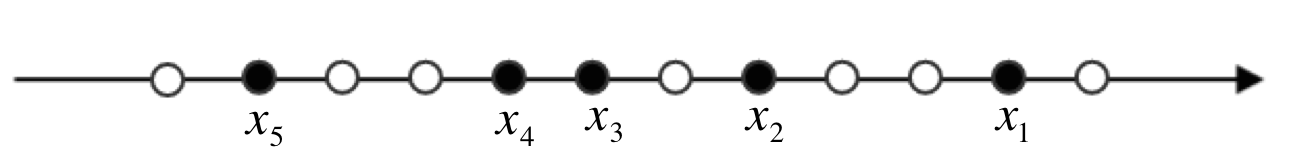
\includegraphics[width=0.5\textwidth]{q-TASEP}
	\caption[An illustration of q-TASEP]
	{An illustration of q-TASEP. The jump rate of the particle $x_2$ is given by $a_2(1-q^2)$, while that of the particle $x_4$ is $0$.}
	\label{fig:q-TASEP}
\end{figure}

It's worth noting that the ordering of the particles remains unchanged throughout the process. Note also that in the definition of q-TASEP, numbering of the particles starts with $1$. However, to facilitate our discussion, we could have added a virtual partical $x_0$ with $x_0 = \infty$ so that the jump rate of $x_1$ is also equal to $a_1 (1-q^{x_0(t) - x_1(t) + 1}) = a_1$. 

It can be easily seen that dynamics of the right most $N$ particles, i.e., particle $x_1$, $x_2$, $\dots$, $x_N$, is independent from those to the left of them, i.e., $x_{N+1}$, $x_{N+2}$, $\dots$ Therefore, from now onwards, we will be focusing on the study of q-TASEP with $N$ particles, with configuration $x_1(t) > x_2(t) > \dots > x_N(t)$. We could then define our state space as $$X^N = \{\vec{x}=(x_0,x_1,\dots, x_N) \in \{\infty \} \times \mathbb{Z}^N : \infty = x_0 > x_1 > \dots > x_N \}.$$

For q-TASEP with $N$ particles, the infinitesimal generator of $\vec{x}(t)$ acting on suitable function $f: X^N \rightarrow \mathbb{R}$, denoted by $L^{q-TASEP} f$, is given by $$(L^{q-TASEP} f) (\vec{x}) = \sum_{i=1}^{N} a_i (1-q^{x_{i-1} - x_i - 1}) (f(\vec{x}_i^{+}) - f(\vec{x})),$$ where $\vec{x}_i^{+}$ denotes the configuration of the q-TASEP with particle $x_i$ jumps to the right by $1$ position, i.e., $\vec{x}_i^+ = (x_0, x_1, \dots, x_{i-1}, x_i+1, x_{i+1}, \dots, x_N)$. This follows from the fact that for $t$ small, there is only $1$ chance for one of the $N$ particles to jump according its own jump rate.

\section{Initial data for q-TASEP}
For a q-TASEP to be well defined, additional to the dynamics of q-TASEP described in Section \ref{sec:intro-qtasep}, we also need an initial configuration of the process, called initial data. In this paper, we focus on two types of initial data, namely, the step initial data and the half stationary initial data. 

Step initial data is defined as the configuration of $x_i(0) = -i$ for $1 \le i \le N$. For half stationary initial data, we define q-Geometric distribution. 

\begin{definition}
\label{def:qgeo}
For $\alpha \in [0,1)$, we say that a random variable $X$ follows the q-Geometric distribution with parameter $\alpha$ [written as $X \sim qGeo(\alpha)$] if $$\mathbb{P}(X = k) = (\alpha;q)_{\infty} \frac{\alpha^k}{(q;q)_k},$$ where $(a;q)_n = (1-a)(1-aq)(1-aq^2)\dots(1-aq^{n-1})$ and $(a;q)_{\infty} = (1-a)(1-aq)(1-aq^2)\dots$
\end{definition}

Let $X_i \sim qGeo(\alpha/a_i)$ for $1 \le i \le N$ be $N$ independent q-Geometric random variables. Then the half stationary initial condition is defined recursively by first setting $x_1(0) = -1 + X_1$ and letting $x_i(0) = -1 + x_{i-1}(0) + X_i$ for $i > 1$. Note that when $\alpha = 0$, the step initial data is recovered.

\section{q-TASEP for a few particles}
The main goal for the study of q-TASEP in this thesis is to identify an exact formula for the distribution of the particle positions, $\mathbb{P}(x_N(t) = m)$ for $m \in \mathbb{Z}$ with step and half stationary initial data. In this section, we provide some intuitions of how this problem can be approached via elementary methods for q-TASEP of $1$ and $2$ particles, thereby illustrating how the complexity grows for $N$ large. 

\subsection{q-TASEP with $1$ particle}
In this section we focus on the q-TASEP with only $1$ particle denoted by $x_1$ starting at position $x_1(0) = 0$. Let $T_i$, $i = 1,2,\dots$ be independent and identically distributed exponential random variables with parameter $1$ denoting the time between the $(i-1)th$ and the $ith$ jump. For $m \in \mathbb{Z}_{\ge 0}$, define $$a_m = \mathbb{P}(x_1(t) \le m) = \mathbb{P}(\sum_{i=1}^{m+1} T_i > t)$$ such that $\mathbb{P}(x_1(t) = m) = a_m - a_{m-1}$ for $m \ge 1$ and $\mathbb{P}(x_1(t) = 0) = a_0 = e^{-t}$. Since $T_i \sim exp(1)$, $\sum_{i=1}^{m} T_i \sim Erlang(m,1)$ and therfore, by the density function of Erlang distribution, $$1 - a_m = \int_0^t \frac{s^m}{m!} e^{-s} ds.$$ 

\begin{proposition}
For q-TASEP with one particle $x_1$ with jump rate parameter $a_1 = 1$ and initial profile at $x_1(0) = -1$, we have that $\mathbb{E}[x_1(t)+1] = t$ and $\mathbb{E}[q^{x_1(t)+1}] = e^{(q-1)t}$.
\end{proposition}

\begin{proof}
From the notations above, we have that $\mathbb{P}(x_1(t) = m) = c_m - c_{m-1}$, where $c_m$ is defined by $c_m = 1 - \int_0^t \frac{s^m}{m!} e^{-s} ds$. Therefore, we have
\begin{align*}
\mathbb{E}[x_1(t)] &=  \lim_{n \to \infty} ((1-c_0) + (1-c_1) + ... + (1-c_{n-1}) - n ( 1-c_n))\\
  						&= \lim_{n \to \infty} (\int_{0}^{t} e^{-s}  (\sum_{i=0}^{n-1} \frac{s^i}{i!}) ds) +\lim_{n \to \infty} (n \times \int_{0}^{t} \frac{s^n}{n!} e^{-s} ds)\\
						&=  \int_{0}^{t} e^{-s} \lim_{n \to \infty} (\sum_{i=0}^{n-1} \frac{s^i}{i!}) ds + 0\\
						&=  \int_{0}^{t} e^{-s} e^s dt\\
						&= t
\end{align*}
Moreover, $\mathbb{E}[q^{x_0(t)}]$ can be computed as below: 
\begin{align*}
\mathbb{E}[q^{x_0(t)}] &= \lim_{n \to \infty} (q^0  c_0 + \sum_{i=1}^{n} q^i (c_i - c_{i-1}) )\\
											 &= \lim_{n \to \infty} (-(1-q) (\sum_{i=0}^{n-1} q^i (1-a_i)) - q^n (1-c_n) + 1)\\
											 &= - (1-q) \lim_{n \to \infty} ( \int_{0}^{t} e^{-s} \sum_{i=0}^{n-1} q^i \frac{s^i}{i!} ds) - \lim_{n \to \infty} \int_0^t q^n \frac{s^n}{n!} ds + 1\\
											 &=  - (1-q) \int_0^t e^{-s }  \lim_{n \to \infty} \sum_{i=0}^{n-1} q^i \frac{s^i}{i!} ds- \lim_{n \to \infty} \int_0^t q^n \frac{s^n}{n!} ds + 1\\
				     					 &=  - (1-q) \int_0^t e^{-s } e^{qs}  ds -\lim_{n \to \infty}  \int_0^t q^n \frac{s^n}{n!} ds + 1\\
				     					 &= e^{(q-1)t}.
\end{align*}
\end{proof}

\subsection{q-TASEP with $2$ particles}
Elementary methods similar to the one adopted for the one-particle system were applied for the $2$ particles system, and it was realized that the computation grew so complicated that nearly no conclusions was reached. Therefore, a different approach, namely the Komogorov Equation, was used to carry out the computation. Although no final conclusion was reached either at the end, some interesting results were found. 

Let us consider the two particles labeled as $x_1$ and $x_2$ starting at the initial positions that $x_1(0) = 0$ and $x_2(0) = a << 0$. Let $\mathbb{P}_{k,j}(t) = \mathbb{P}(x_1(t) = k, x_2(t) = j)$. We begin by giving the Komogorov Equation for the problem:
$$\frac{d}{dt} \mathbb{P}_{k,j}(t) = - \mathbb{P}_{k,j}(t) - (1-q^{k-j-1})\mathbb{P}_{k,j}(t) + (1-q^{k-j})\mathbb{P}_{k,j-1}(t) + \mathbb{P}_{k-1,j}(t)$$
with base cases  $\mathbb{P}_{k,j}(t) = 0$ if $j < a$ or $k < 0$ or $j \ge k$.\\
We will be applying induction on $k$ and $j$ separately, starting by iterating through $k = 0, 1, 2, \dots$. The result is stated as a proposition.
\begin{proposition}
With the notations and setting introduced above, for $m \ge 1$
 $$ \mathbb{P}_{m,a}(t) =\frac{1}{2 \pi i} \oint_{all poles} \frac{e^{(-2+z)t}}{(z-q^{-a-1})(z-q^{-a})...(z-q^{-a+m-1})} dz.$$
\end{proposition}
\begin{proof}
We will not be showing a complete proof here. Rather, we give some calculations for some base cases to check that the proposition is correct and provide some intuitions. \\
\textbf{Case 1}: For $k=0,j=a<0$, we have $$\frac{d}{dt} \mathbb{P}_{0,a}(t) + (2-q^{-a-1}) \mathbb{P}_{0,a}(t) = 0$$
 Solving this equation gives $$\mathbb{P}_{0,a}(t) = c e^{-(2-q^{-a-1})t}$$
 Notice that $\mathbb{P}_{0,a}(0) = 1$, then $c=1$. Therefore $$\mathbb{P}_{0,a}(t) = e^{-(2-q^{-a-1})t} = \frac{1}{2 \pi i} \oint_{all poles} \frac{e^{(-2+z)t}}{z-q^{-a-1}} dz$$
 \textbf{Case 2}: For $k=1, j=a<0$, we have $$\frac{d}{dt} \mathbb{P}_{1,a}(t) + (2-q^{-a}) \mathbb{P}_{1,a}(t) = e^{-(2-q^{-a-1})t}$$
 Therefore, $$\frac{d}{dt} [e^{(2-q^{-a})t} \mathbb{P}_{1,a}(t)] = e^{(q^{-a-1} - q^{-a})t}$$
 Solving this equation we have $$ \mathbb{P}_{1,a}(t) = \frac{e^{-(2-q^{-a-1})t}}{q^{-a-1} - q^{-a}} + c e^{-(2-q^{-a})t}$$
 Note that $\mathbb{P}_{1,a}(0) = 0$, we have $c = -\frac{1}{q^{-a-1} - q^{-a}}$ and therefore $$\mathbb{P}_{1,a}(t) = \frac{1}{q^{-a-1} - q^{-a}} (e^{-(2-q^{-a-1})t} - e^{-(2-q^{-a})t})$$
 In \textbf{contour integral} form, it can also be written as $$\mathbb{P}_{1,a}(t) =\frac{1}{2 \pi i} \oint_{all poles} \frac{e^{(-2+z)t}}{(z-q^{-a-1})(z-q^{-a})} dz$$
 \textbf{Case 3}: For $k=2, j=a<0$, we have $$\frac{d}{dt} \mathbb{P}_{2,a}(t) + (2-q^{1-a}) \mathbb{P}_{2,a}(t) = \mathbb{P}_{1,a}(t)$$
 Solving this equation gives 

 \begin{align*}
  \mathbb{P}_{2,a}(t) &= \frac{e^{(-2+q^{-a-1})t}}{ (q^{-a-1} - q^{-a})(q^{-a-1} - q^{1-a}) } - \frac{ e^{(-2+q^{-a})t} }{ (q^{-a-1} - q^{-a}) (q^{-a} - q^{1-a}) }\\
  & \quad + \frac{e^{(-2+q^{-a+1})t}}{ (q^{-a-1} - q^{-a+1})(q^{-a} - q^{-a+1}) } \\
  &=\frac{1}{2 \pi i} \oint_{all poles} \frac{e^{(-2+z)t}}{(z-q^{-a-1})(z-q^{-a})(z-q^{-a+1})} dz
 \end{align*}
\end{proof}
Next, we investigate the cases $k = 0, j = a, (a+1), \dots, -1$. The result is stated as the following proposition.
\begin{proposition}
With the notations and setting introduced above, for $k = 0, j = a+n$, $0 \le n < a$, we have \\
\begin{align*}
\mathbb{P}_{0,a+n} (t) &= \frac{(1-q^{-a-1})(1-q^{-a-2})...(1-q^{-a-n})}{2 \pi i} \\
& \quad \times \oint_{all poles} \frac{e^{(-2+z)t}}{(z-q^{-a-1})(z-q^{-a-2})...(z-q^{-a-n-1})} dz.
\end{align*}
\end{proposition}

\begin{proof}
Again, we will only be providing some intuitions regarding the equality. \\
For $k=0, j=a+1$, we have $$\frac{d}{dt} \mathbb{P}_{0,a+1}(t) + (2-q^{-a-2}) \mathbb{P}_{0,a+1}(t) = (1-q^{-a-1}) \mathbb{P}_{0,a}(t)$$
 Solving this equation gives 

 \begin{align*}
 \mathbb{P}_{0,a+1} (t) &= \frac{1-q^{-a-1}}{q^{-a-1} - q^{-a-2}} (e^{-(2-q^{-a-1})t} - e^{-(2-q^{-a-2})t})\\
 &= (1-q^{-a-1}) \frac{1}{2 \pi i} \oint_{all poles} \frac{e^{(-2+z)t}}{(z-q^{-a-1})(z-q^{-a-2})} dz
 \end{align*}
\end{proof}

More general application of induction on both $k$ and $j$ together was carried out and didn't reach any elegant results as the ones mentioned above. Therefore, the elementary calculation for the q-TASEP model was stopped and the focus was then turned to studying the duality approach. However, such calculations demonstrate how fast the complexity grows with the number of particles considered, and they were also important as they provided essential fundamental understanding of the model. 

\section{Introduction to q-TAZRP}
Next, we introduce another Markov process called q-TAZRP, short for q-deformed totally asymmetric zero range process. q-TAZRP on an interval $\{0,1,...,N\}$ is a continuous time, discrete space Markov process $\vec{y}(t)$ with state space $$Y^N = (\mathbb{Z}_{\ge 0})^{N+1}$$ subject to the condition of $\sum_{i=0}^{N} y_i(t) = \sum_{i=0}^{N} y_i(0)$ $\forall$ $t\in\mathbb{R}_{\ge 0}$. Dynamics of a q-TAZRP is defined as the following:
\begin{itemize}
\item For each $i \in \{1,2,\dots,N\}$, $y_i(t)$ decreases by $1$ and $y_{i-1}(t)$ increases by $1$ simultaneously according to a rate function given by $g_i(k) = a_i (1-q^{y_i(t)})$.
\item All changes occur independently for each site according to exponential clocks.
\item $y_0$ is always non-decreasing.
\end{itemize}

\begin{figure}
	\centering
	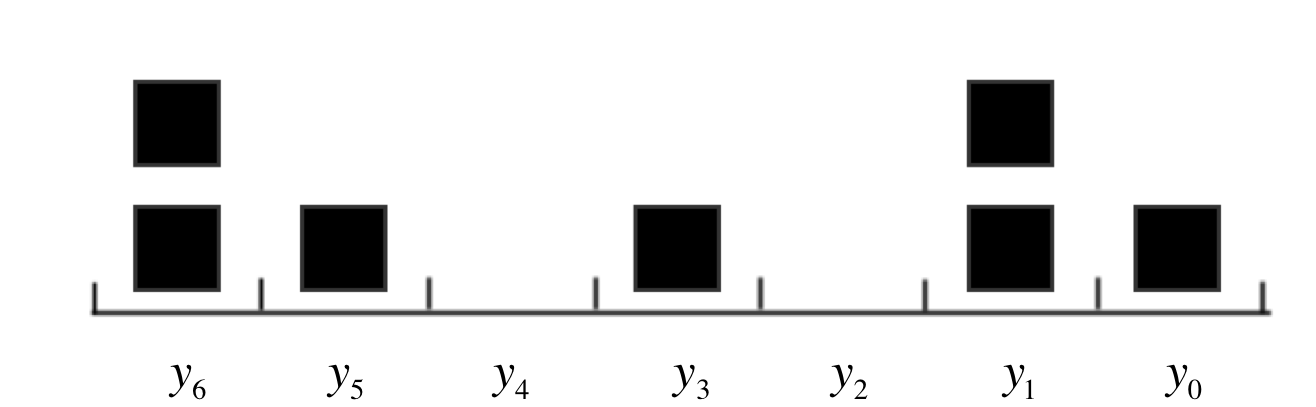
\includegraphics[width=0.75\textwidth]{q-TAZRP}
	\caption[An illustration of q-TAZRP]
	{An illustration of q-TAZRP. Rate function for site $y_1$ is given by $a_1 (1-q^2)$.}
	\label{fig:qTAZRP}
\end{figure}

A natural interpretation of the q-TAZRP is given in Figure \ref{fig:qTAZRP}, where a total of $\sum_{i=0}^{N} y_i(0)$ particles occupy the $N$ sites ordered in such a way that $y_i$ is to the left of $y_{i-1}$ for $i = 1,2,\dots,N$. The changes in the definition then refer to a jump of the top particle at site $y_i$ to the site $y_{i-1}$. Note then that no particle leaves site $0$.

It can be shown that the infinitesimal generator of $\vec{y}(t)$ acting on a suitable function $h:Y^N \rightarrow \mathbb{R}$, denoted as $L^{q-TAZRP} h$, is given by $$(L^{q-TAZRP} h)(\vec{y}) = \sum_{i=1}^{N} a_i (1-q^{y_i}) (h(\vec{y}^{i,i-1}) - h(\vec{y})),$$ where $\vec{y}^{i,i-1}$ represents the configuration of $(y_0, \dots, y_{i-2}, y_{i-1}+1, y_i - 1, y_{i+1}, \dots, y_N)$.

Lastly, we present another notation, $\vec{n} \in W^k_{>0}$, for the states of a q-TAZRP, where $W^k_{>0} = \{(n_1,n_2,\dots,n_k) \in (\mathbb{Z}_{>0})^k : n_1 \ge n_2 \ge \dots \ge n_k \ge 0 \}$. The vector $\vec{n}(\vec{y})$ for any state $\vec{y}$ of the q-TAZRP is given by $$y_i = \left| \{ n_j : n_j = i \} \right|.$$ The intuition is that while $y_i$ in $\vec{y}$ denotes the number of particles at site $i$, $n_j$ in $\vec{n}$ denotes the positioin of Particle $j$ ordered according to decreasing site locations. Take the configuration in Figure \ref{fig:qTAZRP} for example. Its representation in $\vec{y}$ is given by $\vec{y} = (1,2,0,1,0,1,2)$, while in $\vec{n}$ it is represented as $\vec{n} = (6,6,5,3,1,1,0)$. 

\chapter{Duality and Nested Contour Integral Ansatz Solution}
In this chapter, we recall the definition of duality between two Markov process defined in \cite{interacting-particle-system}. Then we prove the duality between q-TASEP and q-TAZRP. We then conclude by giving an ansatz solution for q-TASEP with step initial data as well as half stationary initial data. 

\section{Duality}
a
\section{Duality between q-TASEP and q-TAZRP}
a
\section{Evolution Equation Systems}
a
\section{Nested Contour Integral Solution}
a
\appendix
\chapter{Tables}

\begin{table}
\caption{Armadillos}
\label{arm:table}
\begin{center}
\begin{tabular}{||l|l||}\hline
Armadillos & are \\\hline
our	   & friends \\\hline
\end{tabular}
\end{center}
\end{table}

\clearpage
\newpage

\chapter{Figures}

\vspace*{-3in}

\begin{figure}
\vspace{2.4in}
\caption{Armadillo slaying lawyer.}
\label{arm:fig1}
\end{figure}
\clearpage
\newpage

\begin{figure}
\vspace{2.4in}
\caption{Armadillo eradicating national debt.}
\label{arm:fig2}
\end{figure}
\clearpage
\newpage

%% This defines the bibliography file (main.bib) and the bibliography style.
%% If you want to create a bibliography file by hand, change the contents of
%% this file to a `thebibliography' environment.  For more information 
%% see section 4.3 of the LaTeX manual.
\begin{singlespace}
\bibliography{main}
\bibliographystyle{plain}

\begin{thebibliography}{9}

\bibitem{duality2014}
  A.Borodin, I. Corwin, and T. Sasamoto,
  \emph{From duality to determinants for q-TASEP and ASEP},
  Annals of Probability 2014,
  Vol. 42, No. 6, 2314-2382,
  2014,
  arXiv:1207.5035.

\bibitem{macdonald2014}
  A.Borodin, I. Corwin,
  \emph{Macdonald processes},
  Probability Theory and Related Fields,
  2014,
  arXiv:1111.4408.

\bibitem{generator-duality}
  A. Vo\ss -B\"o hme, W. Schenk and A.-K. Koellner,
  \emph{On the equivalence between Liggett duality of Markov processes and the duality relation between their generators},
  Markov Processes and Related Fields,
  2011

\bibitem{phase2015}
  G. Barraquand,
  \emph{A phase transition for q-TASEP with a few slower particles},
  Stochastic Processes and Their Applications 125 (2015),
  pp. 2674-2699,
  2015,
  arXiv:1404.7409.

\bibitem{symmetrization}
  I.G. Macdonald,
  \emph{Symmetric functions and Hall polynomials},
  2nd edition, 
  Oxford University Press,
  New York,
  1999

\bibitem{interacting-particle-system}
  Liggett, T. M.,
  \emph{Interacting Particle Systems},
  Springer,
  Berlin,
  2005,
  MR2108619.

\bibitem{asymptotics2013}
  P. L. Ferrari, B. Vet\H o,
  \emph{Tracy-Widom asymptotics for q-TASEP},
  Ann. Inst. H. Poincar\' e Probab. Stat.,
  2013,
  arXiv:1310.2515.

\end{thebibliography}

\end{singlespace}

\end{document}

